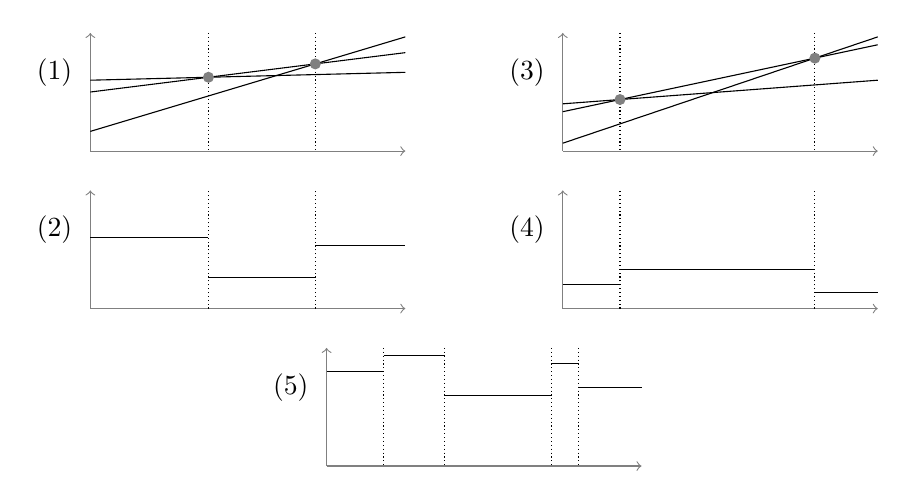
\begin{tikzpicture}
	\tikzstyle{axes} = [->,gray,thin]
	\tikzstyle{boundary} = [thin,densely dotted]

	% step 1
	\node [anchor=east,left=3pt] at (0,1) {(1)};
	\draw[axes] (0,0) -- +(0,1.5);
	\draw[axes] (0,0) -- +(4,0);
	\draw (0,0.25) node (a 1){} -- (4,1.45) node (b 1){};
	\draw (0,0.75) node (a 2){} -- (4,1.25) node (b 2){};
	\draw (0,0.9)node (a 3){} -- (4,1) node (b 3){};

	\path (intersection of a 1--b 1 and a 2--b 2) coordinate (bound 1);
	\draw[boundary] (bound 1 |- 0,1.5) -- (bound 1 |- 0,0);

	\path (intersection of a 3--b 3 and a 2--b 2) coordinate (bound 2);
	\draw[boundary] (bound 2 |- 0,1.5) -- (bound 2 |- 0,0);
	
	\fill[gray] (bound 1) circle (2pt);
	\fill[gray] (bound 2) circle (2pt);

	% step 2
	\node [anchor=east,left=3pt] at (0,-1) {(2)};
	\draw[axes] (0,-2) -- +(0,1.5);
	\draw[axes] (0,-2) -- +(4,0);

	\draw[boundary] (bound 1 |- 0,-2) -- (bound 1 |- 0,-0.5);
	\draw[boundary] (bound 2 |- 0,-2) -- (bound 2 |- 0,-0.5);

	\draw (0,-1.1) -- (0,-1.1 -| bound 2);
	\draw (4,-1.2 -| bound 1) -- (4, -1.2);
	\draw (bound 2 |- 0,-1.6) -- (bound 1 |- 0,-1.6);
	
	% step 3
	\node [anchor=east,left=3pt] at (6,1) {(3)};
	\draw[axes] (6,0) -- +(0,1.5);
	\draw[axes] (6,0) -- +(4,0);
	\draw (6,0.1) node (a 4){} -- (10,1.45) node (b 4){};
	\draw (6,0.5) node (a 5){} -- (10,1.35) node (b 5){};
	\draw (6,0.6) node (a 6){} -- (10,0.9) node (b 6){};

	\path (intersection of a 4--b 4 and a 5--b 5) coordinate (bound 3);
	\draw[boundary] (bound 3 |- 0,1.5) -- (bound 3 |- 0,0);

	\path (intersection of a 6--b 6 and a 5--b 5) coordinate (bound 4);
	\draw[boundary] (bound 4 |- 0,1.5) -- (bound 4 |- 0,0);
	
	\fill[gray] (bound 3) circle (2pt);
	\fill[gray] (bound 4) circle (2pt);


	% step 4
	\node [anchor=east,left=3pt] at (6,-1) {(4)};
	\draw[axes] (6,-2) -- +(0,1.5);
	\draw[axes] (6,-2) -- +(4,0);
	
	\draw[boundary] (bound 3 |- 0,-2) -- (bound 3 |- 0,-0.5);
	\draw[boundary] (bound 4 |- 0,-2) -- (bound 4 |- 0,-0.5);

	\draw (6,-1.7) -- (0,-1.7 -| bound 4);
	\draw (10,-1.8 -| bound 3) -- (10, -1.8);
	\draw (bound 4 |- 0,-1.5) -- (bound 3 |- 0,-1.5);

	% step 5
	\begin{scope}[xshift=3cm,yshift=-4cm]
		\node [anchor=east,left=3pt] at (0,1) {(5)};
		\draw[axes] (0,0) -- +(0,1.5);
		\draw[axes] (0,0) -- +(4,0);

		\path (0,0.25) node (a 1){} -- (4,1.45) node (b 1){};
		\path (0,0.75) node (a 2){} -- (4,1.25) node (b 2){};
		\path (0,0.9) node (a 3){} -- (4,1) node (b 3){};

		\path (intersection of a 1--b 1 and a 2--b 2) coordinate (bound 1);
		\draw[boundary] (bound 1 |- 0,1.5) -- (bound 1 |- 0,0);

		\path (intersection of a 3--b 3 and a 2--b 2) coordinate (bound 2);
		\draw[boundary] (bound 2 |- 0,1.5) -- (bound 2 |- 0,0);

		\path (0,0.1) node (a 4){} -- (4,1.45) node (b 4){};
		\path (0,0.5) node (a 5){} -- (4,1.35) node (b 5){};
		\path (0,0.6) node (a 6){} -- (4,0.9) node (b 6){};

		\path (intersection of a 4--b 4 and a 5--b 5) coordinate (bound 3);
		\draw[boundary] (bound 3 |- 0,1.5) -- (bound 3 |- 0,0);

		\path (intersection of a 6--b 6 and a 5--b 5) coordinate (bound 4);
		\draw[boundary] (bound 4 |- 0,1.5) -- (bound 4 |- 0,0);

		\draw (bound 2 |- 0,0.9) -- (bound 1 |- 0,0.9);
		\draw (bound 2 |- 0,1.4) -- (bound 4 |- 0,1.4);
		\draw (bound 1 |- 0,1.3) -- (bound 3 |- 0,1.3);

		\draw (0,1.2) -- (0,1.2 -| bound 4);
		\draw (4,1.0 -| bound 3) -- (4, 1.0);
	\end{scope}
	
\end{tikzpicture}